\documentclass[border=2pt]{standalone}
\usepackage{tikz}
\usetikzlibrary{arrows.meta}

\begin{document}
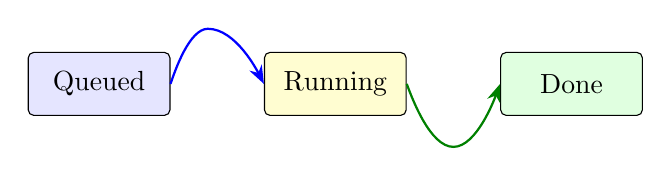
\begin{tikzpicture}[
  >=Stealth,
  stage/.style={draw, rounded corners=2pt, minimum width=18mm, minimum height=8mm},
  arched/.style={parabola height=7mm, bend pos=.4}
]
  \node[stage, fill=blue!10] (queue) at (0,0) {Queued};
  \node[stage, fill=yellow!18] (worker) at (3,0) {Running};
  \node[stage, fill=green!12] (done) at (6,0) {Done};

  \draw[->, thick, blue] (queue.east) parabola[arched] (worker.west);
  \draw[->, thick, green!50!black]
    (worker.east) parabola bend (4.5,-.8) (done.west);
\end{tikzpicture}
\end{document}
